\thesischapterexordium

\section{研究工作的背景与意义}
文本分类是自然语言处理较为关键的一项任务,比如邮件分类、观点挖掘、情感分析等\citing{sculley2007relaxed,saif2016contextual}。主要是通过对已知的一些文本进行训练学习,建立一个模型,挖掘文本中的深层次含义以及潜在规律,从而实现对未知文本的预测。例如,对于情感分类模型来说,通过输入用户的一句话或者一段话,实现对这段文本的分析,预测用户的情感,是消极还是积极。
随着互联网的飞速发展,网络中存在着大量的文本数据,尤其是类似于美团、豆瓣等数字平台上充满了用户行为留下来的大量文本,如富有感情色彩的评论,对电影的点评、对美食的评价。以及各大新闻论坛也包含了多种多样的新闻主题,例如政治类、财经类、娱乐类。从这些海量数据中挖掘出用户的情感,有助于精准地刻画用户,从而辅助平台进行针对性的提供服务。同时,用户对某一事项的不同方面进行评价,有利于对这些方面的不足之处进行改进以提升用户感知。过去文本分类涉及了许多人工操作,例如新闻主题分类,依赖于工作人员的主观判断,将对应的新闻主体分类至对应的主题类目下。随着文本的不断累积,加上每天大量的新增文本,为手工分类带来了巨大挑战,极大的增加了人力成本。自动化的文本分类出现,能够显著降低劳动成本,提升工作效率。
方面级的情感分类是指针对一段文本中指向的一个具体方面进行评价。例如一句话“这家餐馆的菜品很好吃,但是服务不太好”。这句话中主要提到了两个方面,一个是“菜品”,一个是“服务”。
并且针对这两个方面有着不同的评价,分别是“很好吃”和“不太好”。方面级情感分类模型实现的就是对于“菜品”这个方面进行打分评价。
相比于一般的文本分类针对的是一段文本或一句话进行的分类,方面级情感分类更加细分,需要捕捉到关键词的情感,更加注重于对某个关键词所表达的含义。
互联网的高速发展,各大平台将会产生大量的文本信息,自动化的分类文本,通过用户发布的文本内容,精准地刻画用户情感,从而支持业务决策,正是本论文研究的意义和价值所在。
传统的机器学习方法需要大量的手工提取特征的方式,增加了研究者的负担。而一些采用深度学习的方式在文本处理领域略有不足,例如很多算法忽略了文本的整体信息以及文本在语料库中的统计信息。尤其是在对于方面级目标词与文本内容之间关系的捕捉,很多模型仍有改进空间,因此文本分类任务的效率和准确度还有待提高。       
本学位论文研究基于图模型的文本分类算法,通过图模型有利于挖掘单词之间的关系信息,通过传递单词之间的信息,不断更新优化单词的向量表示,不断深入挖掘单词之间隐藏的语义信息,同时文本的具体含义与整个语料库的组成也有一定联系,通过图模型捕捉所有文本单词之间的关联有助于提升分类效果。方面级目标词与文本整体的单词之间也应该有较大关联,用户对方面目标所体现的情感应该仅有文本中的部分词有关,而大部分词应该是无关的,本论文希望通过图模型挖掘出这些内在关系,有助于进一步提升文本分类质量。

\section{国内外研究现状}
本论文旨在研究基于图模型的短文本分类算法研究,因此接下来主要介绍图网络模型算法和文本分类算法目前的研究现状。

\subsection{图网络模型算法研究}
在许多领域的数据都很容易转化成图结构。比如蛋白质组学、图像分析、社交网络和自然语言处理等。例如社交网络,每个用户都可以视作一个节点,他们之间的关系就可以构成一条条边,很自然的构成了一个图结构。由于图结构中的节点以及边都可以带有自己的属性信息,同时每个节点以及自己的邻居节点又可以构成一个新的拓扑图结构,因此基于图结构进行分析可以获取得到更加丰富的信息。
图是由节点和边组成的一种结构,节点可以是任意实体对象,比如一个用户,一个地点或是一个单词,而边可以表示为节点之间的特殊联系,比如用户之间的点赞,互相关注等。
\begin{figure}[htb]%\small tbp
	%	\vspace{-0.15cm}
	%	\setlength{\abovecaptionskip}{0pt}
	\setlength{\belowcaptionskip}{0pt}
	\centering
	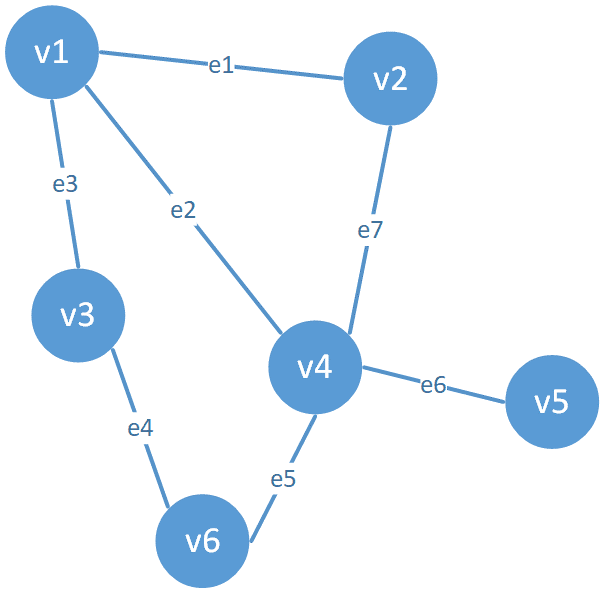
\includegraphics[width=0.4\textwidth]{pic/1-1.png}
	\caption{图结构}
	\label{graphStruc}
\end{figure}
如图\ref{graphStruc}所示是一个基本的图结构。节点之间以边连接,形成一个互相联系的结构。

近些年来,图神经网络已经被广泛应用于学习图的结构化向量表示。已经吸引了越来越多的学者\citing{xu2018powerful,cai2018comprehensive,wu2020comprehensive,zhou2018graph}。图神经网络主要是通过迭代的方式聚集信息,例如某个节点,通过从周围的邻居节点中汇聚信息,然后对信息进行处理,获得自身新的信息表示。再通过多次迭代,不断地更新自身的信息,获得丰富的特征向量表示。

图神经网络也包含多种,不同的网络也常对应不同的应用场景。许多传统的算法往往将图结构的数据压缩为链式结构,或者转换为树状结构,然后再使用链式神经网络(如RNN)或递归神经网络去处理。此时,图中的拓扑结构信息往往会有一定的损失,模型的性能也会受到压。基于此,Li\citing{li2015gated}提出了GGNN(Gated Graph Neural Networks)模型,该模型直接可以使用图结构信息,利用一个GRU模型实现信息的传递。不同节点之间应该具有不同的关系,节点之间的信息传递应该依赖于关系的强弱进行传导,即关系度较高的两个节点之间传递的信息应该占比更多,而关系度低的节点之间应该仅传递较少的信息。而传统的图神经网络往往忽略了这种节点之间信息传递的强弱,Petar Velickovic等人\citing{velivckovic2017graph}提出了一个基于注意力机制的图神经网络GAT(Graph Attention Networks)。该网络利用每个节点的嵌入表示,采用一个自主力机制学到节点之间的权重关系,再通过这种关系进行信息的传递。该网络相比于许多传统的图神经网络模型取得了非常好的效果,但其弊端就是增加了计算量,每次都需要计算相关的权重信息。

图神经网络中,用得较为广泛的就是Kipf\citing{kipf2016semi}等人提出的图卷积神经网络GCN(Graph Convolutional Networks)。GCN是一个多层的神经网络,首先我们定义一个图$G=\left(V,E\right)$,其中$V$代表图上的节点集合,$E$表示为节点之间的边的集合。GCN的包含输入一个节点的向量表示$X$,以及表示图节点关系的邻接矩阵$A$。在每一层神经网络中,每个节点只能从其直接邻居节点处汇聚信息,再加上自身的信息,形成新的表示。随着层次的加深,每个节点可以获取到更远的节点的信息,即获得了多跳的邻居信息。最终模型的输出就是每个节点的新的向量表示。GCN的传播计算如下
\begin{equation}\label{gcnFormula1}
    H^{\left(l+1\right)}=\sigma{{(\hat{D}}^{-\frac{1}{2}}\hat{A}\hat{D}}^{-\frac{1}{2}}H^{\left(l\right)}W^{\left(l\right)})
\end{equation}
\begin{equation}\label{gcnFormula2}
\hat{A}=A+I
\end{equation}
    其中$I$表示为单位矩阵,在原始的邻接矩阵上加上单位矩阵就是为了确保节点每次传递都能考虑到自身的信息。$H^{\left(l\right)}$表示为第l层的节点向量表示,$W^{\left(l\right)}$表示为第l层的参数。$\hat{D}$为$\hat{A}$的度矩阵。

\subsection{文本分类算法研究}
先前大量的文本分类工作主要通过对文本单词特征的提取分析,采用特征工程、机器学习或是深度学习等方式实现文本的分类。本文主要探讨的是两类文本分类,一种是定义为整体文本分类,即直接对于整个文本内容进行分类,例如一段文本。判断它是属于金融类或是娱乐类;一种是方面级情感分类,即是对文本中关注的某一个方面词进行分析,例如一段文本“这个店的服务很好,但是菜品不怎么样”,当方面词为‘服务’时,则分类结果是正面,当方面词为‘菜品’时,分类结果则是负面。两者采用的算法大致都是通用的,只是在部分细节上略有不同,方面级情感分类需要着重关注方面词的情感,在算法的研究上需要进一步精心设计

\subsubsection{整体文本分类算法研究现状}
(1)基于特征工程的算法和单词嵌入

在机器学习中,识别关键的以及找到相关的特征对于分类任务来说至关重要,文本分类任务也是如此。特征工程就是针对对应的文本挖掘其特征表示,最大限度地从原始数据中提取特征以供算法和模型使用。单词嵌入就是将文本中的单词用能代表其内在含义的一个向量进行表征,生成计算机能够识别的方式,进而实现分类任务。

K. Sparck Jones\citing{jones1972statistical}提出了IDF的方法,这个方法可通过与词频连用以减少语料库中隐性常用词的影响,TF便是词频。TF-IDF联合使用,可以作为输入特征进行分类。T. Mikolov等人\citing{mikolov2013efficient,mikolov2013distributed}提出了Word2Vec的方法,用以改进单词的向量表示。它采用了一个两层神经网络的基础架构,采用CBOW或是Skip-gram的模型训练文本单词,挖掘单词语义,将单词嵌入到一个高维的向量表示空间,最终获得每一个单词的一个向量表示。Glove\citing{pennington2014glove}方法也是一种学习单词表示的方法。他与word2vec类似,采用一个大型的语料库进行训练,将单词嵌入到高维空间,实现用一组向量表示单词。Glove方法相比于word2vec,考虑了这种全局词汇的共现信息,并且结合局部上下文窗口的方法的优点。Fastext\citing{joulin2016bag}可以用来学习词向量,也可以用来做一种快速简单有效的文本分类算法。但它也有一个缺点。因为它是对文本中的所有单词向量求和取平均,所以忽略了单词在文本中出现的顺序,可能导致错误的分类结果。

(2) 基于深度学习的算法

深度学习的概念源于人工神经网络的研究,例如含多个隐藏层的多层感知器就是一种深度学习结构。深度学习通过组合低层特征形成更加抽象的高层表示属性类别或特征,以发现数据的分布式特征表示。在自然语言处理方面,已提出了许多模型,尤其是文本分类这一任务上,更是不断有新的方法涌现。

RNN(Recurrent Neural Network)是一类用于处理序列数据的神经网络,广泛应用于各类序列上,备受各类研究者所关注\citing{salehinejad2017recent}。为解决RNN模型的梯度消失问题,提出了LSTM\citing{hochreiter1997long}(Long Short-Term Memory)长短期记忆网络。此外,还有一个RNN变种,GRU\citing{cho2014learning}(Gate Recurrent Unit)模型,它简化了LSTM的门机制,仅有一个重置门和更新门。Bi-LSTM\citing{schuster1997bidirectional}(Bidirectional Recurrent Neural Networks)即双向LSTM网络,考虑了文本的前后两个方向的信息。由Kim等人\citing{kim2014convolutional}提出了Text-CNN模型,将CNN(Convolutional Neural Networks)网络带入了文本处理领域。相继有人提出了RCNN\citing{lai2015recurrent},DRNN\citing{wang2018disconnected},TBCNN\citing{mou2014tbcnn}等基于CNN理论的模型用于文本分类。Liang Yao\citing{yao2019graph}等人提出了基于图卷积神经网络(GCN)的文本分类算法。该模型创新的将图卷积网络应用于文本分类领域,将图神经网络引向了新的方向。近年来最引人瞩目的用于自然语言处理的模型当属于transformer\citing{vaswani2017attention}以及bert\citing{devlin2018bert}模型,将自然语言处理推向了一个新的高度。

\subsubsection{方面级情感分类算法研究现状}
(1)基于传统机器学习的算法

Jiang等人\citing{jiang2011target}在面对应用在推特上的情感分类算法时,首先合并一些独立的特征,其次将一些相关的推文考虑进去作为新的特征,通过这些方式,改进分类算法。Wang等人\citing{wagner2014dcu}采用n-gram特征输入SVM中实现方面级的情感分类。Brychcín等人\citing{brychcin2014uwb}结合利用了约束性方法获取的特征以及非约束性方法获取的特征,将两种方式获得的特征结合通过最大熵分类器实现了方面级情感分类。

(2)基于深度学习的算法

Tang等人\citing{tang2015effective}提出采用LSTM模型捕获目标词与句子之间的关系用以实现方面级情感分类。Xue等人\citing{xue2018aspect}提出了一个采用了门机制的CNN模型,实验结果相比传统的LSTM模型具有更高的准确率以及计算速度。Huang等人\citing{huang2019parameterized}基于CNN模型提出PF-CNN和PG-CNN两种变种用以实现方面级情感分类。Han等人\citing{han2019multi}基于LSTM模型,融合了注意力机制关注方面级目标词以及上下文内容。Li等人\citing{li2019co}利用GRU模型学习文本序列信息,获取每个单词的隐藏层状态表示,此外还利用一个协同注意力机制学习目标是及上下文的向量表示,最后采用一个自注意力机制更新目标词与单词向量之间的权重,获得最终的用以文本分类的向量表示。Huang等人\citing{huang2018aspect}提出了一个AOA(Attention-over-Attention)模型,该模型可以捕捉到方面目标词与文本内容之间的关系信息。Zhang\citing{zhang2019aspect}提出采用图卷积神经网络(GCN)用以学习方面目标单词与文本内容单词之间的关系。首先它将文本通过解析树构建单词之间的关系,利用这种关系构建了一个有向图。该模型采用一个Bi-LSTM模型用以学习文本单词之间的隐藏状态表示,然后将每个单词的隐藏向量表示作为图卷积神经网络模型单词节点的初始化表示,通过几次卷积操作,生成新的向量表示。之后,找到对应的方面目标词在GCN模型的输出向量,再与Bi-LSTM模型的单词隐藏状态向量用注意力机制求得对应的关系权重。最后通过加权求和确定最终的情感向量表示。该方法实现了对句子语法的解析,以及语法对文本情感带来的影响,较为准确地区分了单词之间联系,找到了情感相关词汇,实验结果上相比一些方法有了一定提升。HaoTang\citing{tang2020dependency}结合bert、transformer以及GCN模型,进一步提升了模型的准确率。

\section{主要研究内容}
本文针对基于图模型的文本分类算法进行研究。根据文本内容,将单词作为节点,单词之间的邻接关系或是依赖关系作为边,构成图结构,再采用图模型算法进行文本分析,实现文本分类任务。基于此算法,再引入方面词处理,进一步实现方面级情感分类。
因此,本文主要实现两个方面的研究,一是针对整体文本分类算法进行研究设计,采用图模型算法提升分类任务准确率。二是实现方面级情感分类。基于第一点的研究基础,将方面词考虑进模型,对算法进行改进,实现处理方面级情感分类任务,并以此提高分类准确率。
\subsection{整体文本分类算法设计}
传统的文本分类算法忽略文本在语料库中整体的统计信息,以及单词之间的互相影响。因为单词之间互有关联,尤其是同一个句子中的单词含义应该与整个句子的语义有关,而通常的单词嵌入模型每个词向量仅有一种。本文第三章中将文本中的每个单词视作一个节点,采用滑动窗口构建拓扑图结构,采用图模型将单词之间的信息通过图网络互相传递,重新学得更符合整个句子语义的单词的表示。同时还结合每个单词在整个语料库的统计信息,进一步生成代表整个文本含义的特征向量表示。对于单词向量再采用常规的CNN模型、LSTM模型进行分析,再与单词统计信息学的到特征向量相结合,最终实现文本分类任务。
\subsection{方面级情感分析算法设计}
方面级的目标词与文本内容单词之前应该存在许多联系,如果能够挖掘它们之间的内在关系,便能进一步学到情感信息。本文第四章利用第一点的算法进行扩充,将方面词引入通过图网络模型对单词之间的联系进行挖掘,重新学得文本中每个单词的向量以及方面目标词的向量。同时采用门控机制,进行遗忘和选择记忆不同层节点信息。新学得的词向量更符合文本含义,并且词向量之间也构建了诸多内在联系。接着采用attention机制找出目标词和文本单词之间的关系,即找到最能表达目标词情感的其他单词,最后通过组合这些单词,获得特征向量,实现方面级情感分类任务,提升分类效果。
\section{论文组织结构}
本文共分为五章,每章的主要内容如下:
第一章 绪论。本章主要从根据现实情况分析了文本分类任务的研究背景以及意义,同时简单介绍了图模型相关理论以及文本分类算法以及方面级情感分析算法的国内外研究现状。并对本文的主要研究内容进行了概括。

第二章 相关理论及技术。本章首先介绍了文本的处理方式,以及常用的例如word2vec、glove等单词向量表示学习方法。随后总结了图模型相关理论,着重介绍了GCN网络原理及对关键问题进行了详细描述。接着介绍文本分类任务中常用的门控机制、CNN模型以及注意力机制原理。最后介绍了目前较为流行的Bert模型。

第三章 基于图模型的整体文本分类算法。本章首先介绍了整体文本分类问题的定义,然后对算法的核心思想进行了简单的阐述,接着对算法原理以及算法框架的各个组成部分进行了详细的介绍,
包括图文本的构建方式和超节点的建立方法。随后对实验使用的数据集以及对比方法、评价指标进行了简单介绍,最后通过实验结果证明该模型的有效性。

第四章 基于基于图模型的方面级情感分析算法。本章首先介绍了方面级情感分析任务的描述和定义。接着对本章提出的算法原理进行了详细的阐述。然后介绍了实验数据、对比实验以及验证方法。
最后在多个数据集上进行实验,对比各个方法之间的优劣,通过实验数据表明本章提出的方法在方面级情感分析任务上取得不错的效果。

第五章 总结与展望。总结全文的工作内容,展望未来的研究方向。 
